% Backup slides for Q&A. Fragment: \input from simTIM_ARES26_backup.tex.

\begin{frame}{Backup --- How simTIM relates to other simulators}
\small
\begin{tabular}{@{}p{4.3cm}p{7.0cm}@{}}
  \textbf{Attack graphs} & static reachability; no time, no defender agency\\[1mm]
  \textbf{RL cyber gyms} & turn-based; an action resolves within one step\\[1mm]
  \textbf{Adversary emulation} & executes on real hosts; not what-if\\[1mm]
  \textbf{Temporal security games} & continuous time, but no topology or assets\\[1mm]
  \textbf{Model-based evaluation} & time \emph{and} structure --- closest relatives\\
\end{tabular}
\vspace{3mm}

They model \alert{time without a network}, or a \alert{network without time},
or \alert{reality without what-if}.
simTIM combines them --- and uniquely lets a defence invalidate an attack that
is \emph{already running}.
\end{frame}

\begin{frame}[plain]{Backup --- Why TIM, and not an existing model}
\centering

\includegraphics[page=4, trim=133pt 538pt 131pt 114pt, clip,
                 width=0.92\textwidth]{temporal.pdf}\\[2mm]
{\footnotesize\color{inkGrey}Mann, ``Time is money'', 2025 --- Table 1.
R1--R9 are the requirements of that paper; R8 is action cost and duration.}
\end{frame}

\begin{frame}[plain]{Backup --- Demo fallback}
\centering
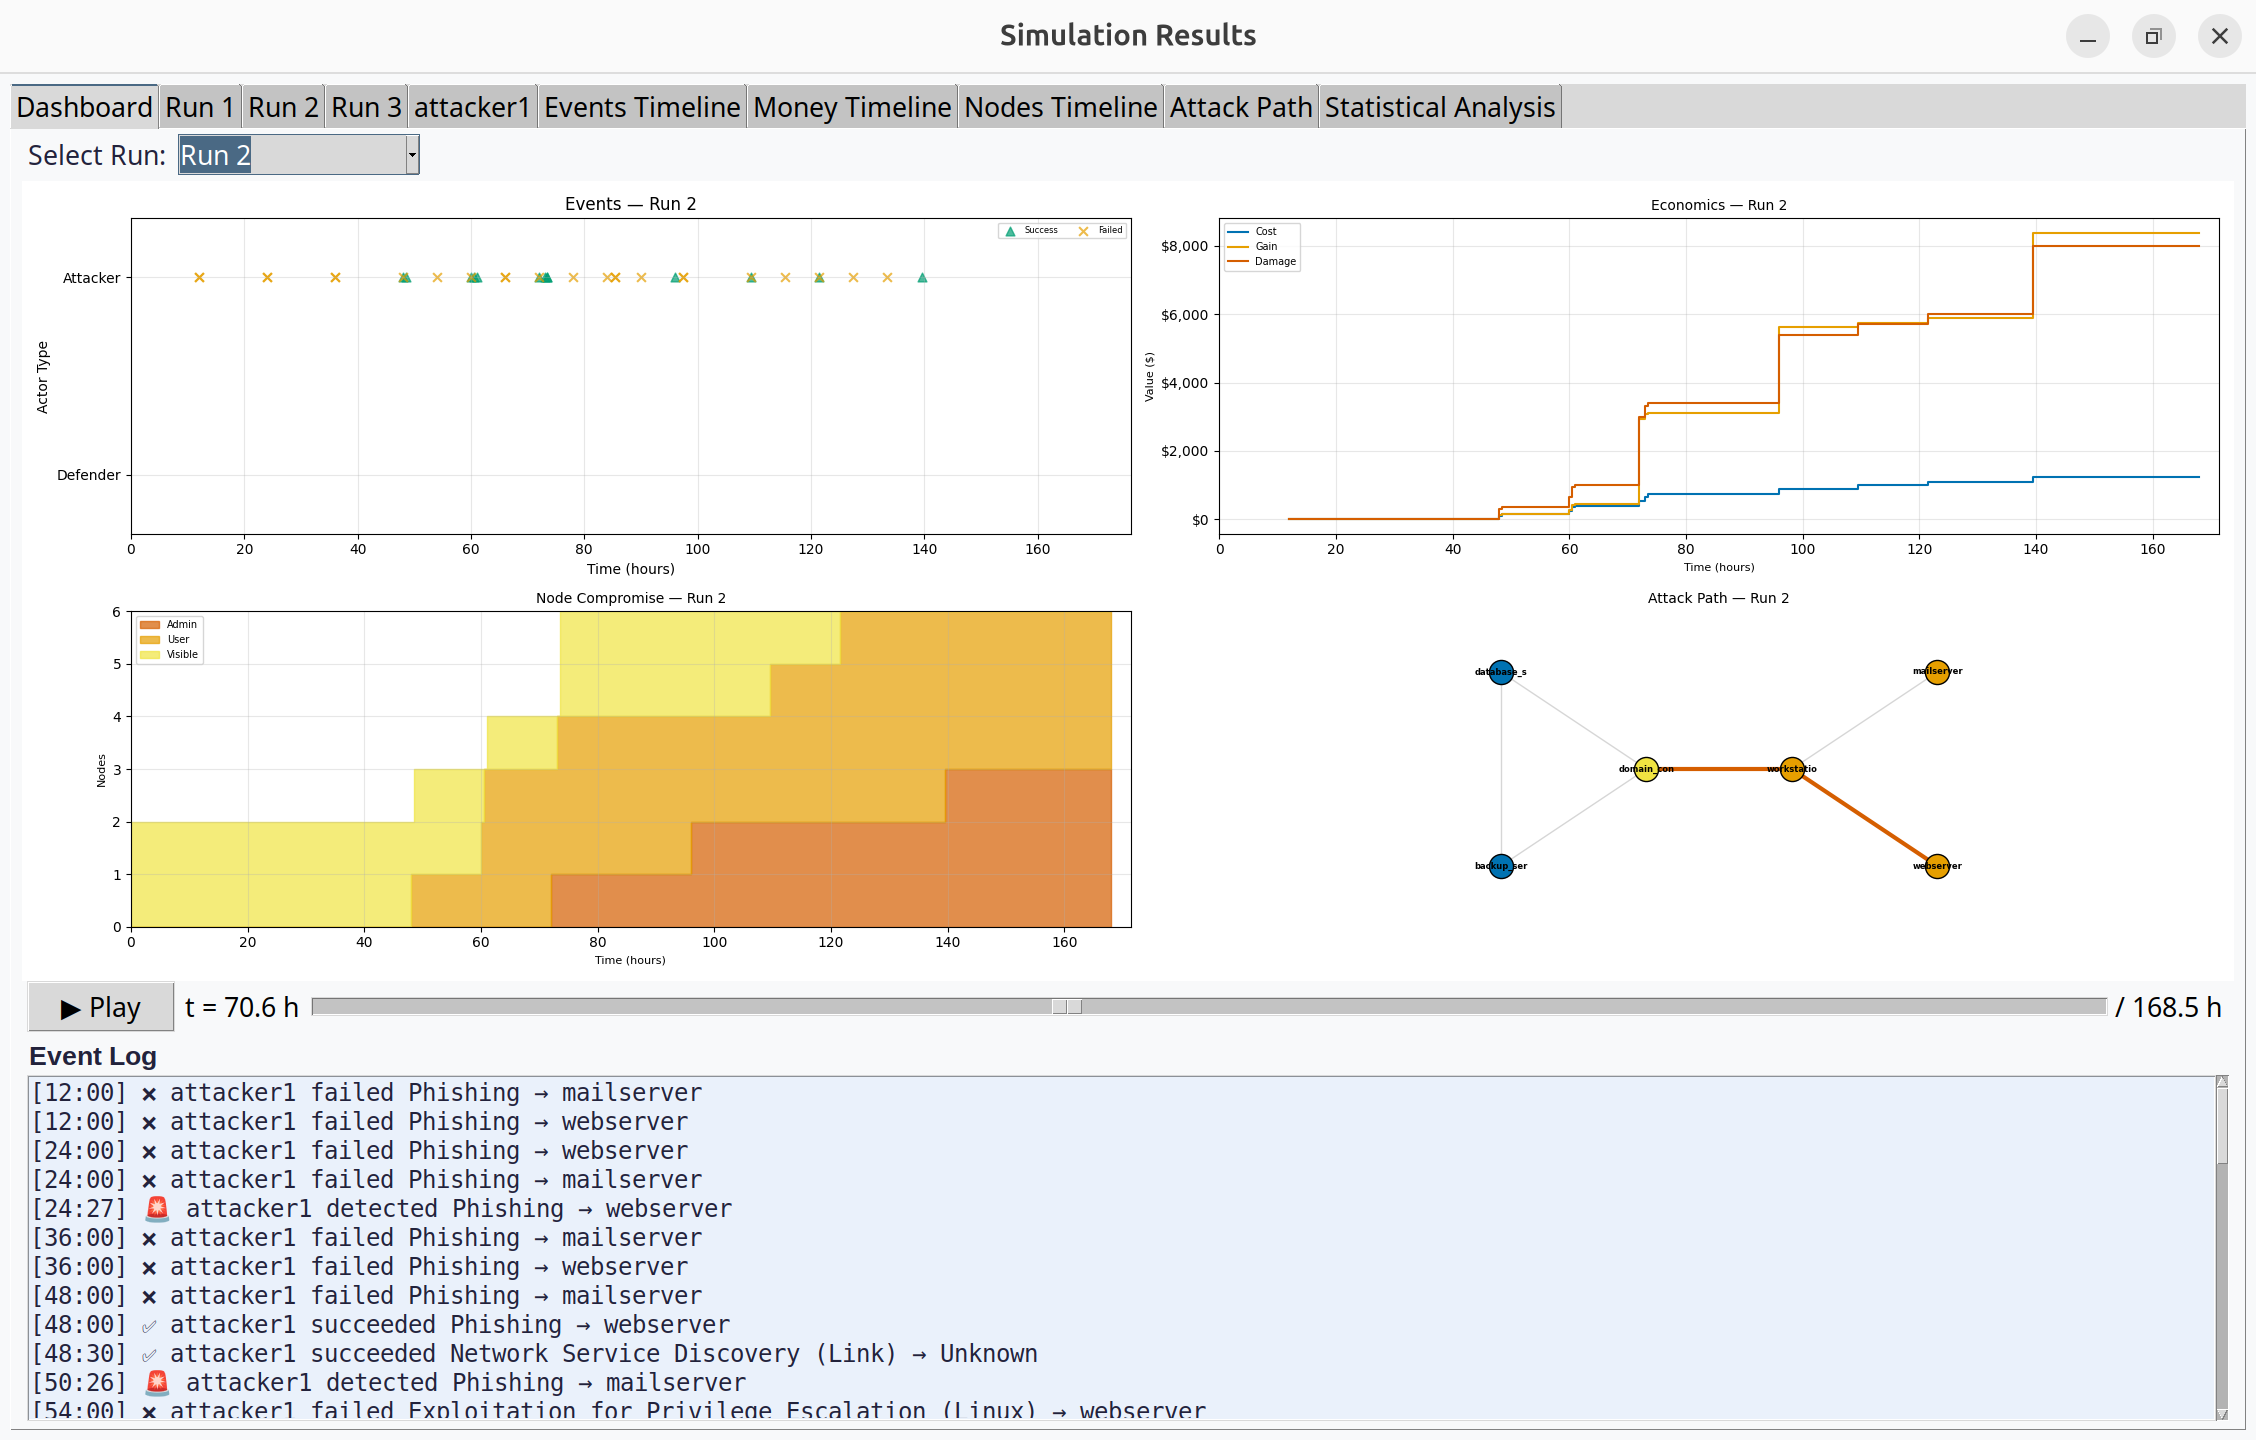
\includegraphics[width=0.86\textwidth]{simTIM_visualization.png}
\end{frame}

\begin{frame}{Backup --- Architecture}
\centering

\includegraphics[width=0.85\textwidth]{architecture.pdf}
\end{frame}

\begin{frame}{Backup --- Detection engines}
\small
Two-step process: a Bernoulli trial with probability $\varrho$ decides
\emph{whether}; a CDF $F_a(t)$ on the normalised progress $t\in[0,1]$ decides
\emph{when}.
\begin{itemize}
  \item \textbf{Uniform}\quad $F_a(t) = t$
  \item \textbf{Early-weighted}\quad $F_a(t) = 1-(1-t)^n$
  \item \textbf{Late-weighted}\quad $F_a(t) = t^n$
\end{itemize}
Timing matters: a late detection may arrive after the damage is done.
New engine $=$ one subclass with three methods.
\end{frame}

\begin{frame}{Backup --- Strategies available today}
\small
\begin{columns}[T]
\begin{column}{0.48\textwidth}
\textbf{Attacker}
\begin{itemize}
  \item escalation --- climb access levels, then scan
  \item greedy --- maximise $p\cdot\text{gain} - \text{cost}$
  \item random --- baseline
\end{itemize}
\end{column}
\begin{column}{0.48\textwidth}
\textbf{Defender}
\begin{itemize}
  \item reactive --- evict and isolate
  \item proactive --- harden
  \item monitoring --- detect and deceive
  \item balanced --- all tactics
\end{itemize}
\end{column}
\end{columns}
\vspace{3mm}
Deliberately simple. The interface, not the heuristics, is the contribution.
\end{frame}

\begin{frame}{Backup --- Validation \& parameters}
\small
\begin{itemize}
  \item simTIM is a \textbf{what-if} tool, not a predictor. It compares
        configurations under identical assumptions.
  \item Parameter sources: CVE/EPSS, MITRE ATT\&CK, internal incident data,
        expert estimate.
  \item Uncertain parameters are \emph{swept}, not guessed --- that is what the
        scenario comparison is for.
  \item Empirical validation against real incident data: future work.
\end{itemize}
\end{frame}

\begin{frame}{Backup --- Scalability}
\small
\begin{itemize}
  \item Discrete-event simulation: cost scales with the number of \emph{events},
        not with simulated time.
  \item Event queue is a binary min-heap (\texttt{heapq}).
  \item An action index makes precondition re-checks cheap when a node changes.
  \item Monte Carlo runs are independent and can be threaded.
  \item Not yet benchmarked on very large enterprise graphs.
\end{itemize}
\end{frame}

\begin{frame}{Backup --- The numbers behind the race}
\small
From the TIM running example:
\begin{itemize}
  \item Attacker wins: $+\$98\,600$ / defender $-\$150\,000$
  \item Defender wins: attacker $-\$600$ / defender $-\$500$
\end{itemize}
\vspace{2mm}
Default durations: 4\,h per attack action, 8\,h for the defensive action.
Detection probability on $n_1$: $\varrho = 0.8$ (Sophos present).
\end{frame}

% ===========================================================================
\begin{frame}[plain]{Backup --- Reproducing the TIM paper result}
\vspace{-1mm}
\begin{columns}[b,onlytextwidth]
  \begin{column}{0.44\textwidth}
    \centering
    % left panel of Fig. 2 in Mann 2025: damage vs. duration of upgrading MySQL
    
\includegraphics[page=13, trim=132pt 587pt 341pt 115pt, clip,
                     width=\linewidth]{temporal.pdf}\\[2mm]
    {\footnotesize\color{inkGrey}TIM, 2025\\ custom code, 2 nodes}
  \end{column}
  \begin{column}{0.54\textwidth}
    \centering
    
\includegraphics[width=\linewidth]{violin_defense_duration.pdf}\\[2mm]
    {\footnotesize\color{inkGrey}simTIM\\ a dropdown, 6 nodes, 125 runs}
  \end{column}
\end{columns}

\vspace{2mm}
\centering
{\large Same finding. \alert{Any model you like.}}
\end{frame}

% ===========================================================================
\begin{frame}[plain]{Backup --- The TIM running example}
\vfill
\centering
\begin{tikzpicture}[
    node distance=1cm,
    box/.style={rectangle, rounded corners=3pt, draw=inkGrey, thick,
                fill=white, minimum width=3.9cm, minimum height=1.15cm,
                align=center, font=\small\bfseries},
    prop/.style={font=\scriptsize, align=left, text=inkGrey},
    scale=1, transform shape]

  % the two nodes
  \node[box] (n1) at (0,0) {Web server\\[-1pt]{\scriptsize $n_1$}};
  \node[box] (n2) at (7,0) {Database\\[-1pt]{\scriptsize $n_2$}};
  \draw[very thick, inkGrey] (n1) -- (n2)
        node[midway, above, font=\scriptsize, text=inkGrey] {link};

  % properties
  \node[prop, below=0.45cm of n1] (p1)
       {Apache Tapestry \textbf{5.7.0}\\ Sophos endpoint protection\\
        \textcolor{atkRed}{exposed to the internet}};
  \node[prop, below=0.45cm of n2] (p2)
       {MySQL \textbf{8.0.28}\\ 10\,000\,000 records\\
        \textcolor{atkRed}{data sensitivity: high}};

  % attacker
  \node[font=\Large] (hack) at (-3.4,0) {\textcolor{atkRed}{$\bigstar$}};
  \node[font=\scriptsize, text=atkRed, below=1mm of hack] {attacker};
  \draw[-{Stealth[length=3mm]}, thick, atkRed, dashed] (hack) -- (n1);
\end{tikzpicture}
\vfill
{\large One known RCE.\quad One database worth \atk{\$150\,000}.\quad
 One question:\\[2mm]
 \textbf{where does my next euro do the most good?}}
\vfill
\end{frame}

% ===========================================================================
% THE KEY SLIDE
% ===========================================================================
{% local styling for the two Gantt frames
\newcommand{\ganttaxis}{%
  \draw[->, inkGrey] (0,-0.85) -- (10.4,-0.85);
  \foreach \x in {0,2,4,6,8,10,12}
     \draw[inkGrey] (0.8*\x,-0.80) -- (0.8*\x,-0.93)
           node[below, font=\tiny, text=inkGrey] {\x};
  \node[font=\tiny, text=inkGrey, anchor=west] at (10.5,-0.85) {h};
}

\begin{frame}[plain]{Backup --- The race, in detail}
\vspace{-1mm}
\centering
\begin{tikzpicture}[
   bar/.style={rectangle, draw=black!55, thick, minimum height=6mm,
               anchor=west, font=\scriptsize, inner sep=2pt},
   lbl/.style={font=\scriptsize\bfseries, anchor=east, text=inkGrey},
   scale=1, transform shape]

% ---------------- PANEL A : fast patch ------------------------------------
\begin{scope}[yshift=3.25cm]
  \node[font=\small\bfseries, anchor=west, text=defBlue] at (-1.9,1.55)
       {Patch takes 4\,h};

  \node[lbl] at (-0.15,0.95) {attacker};
  \node[lbl] at (-0.15,0.25) {defender};

  % attacker bars -- the exploit only ever runs 5h..6h, then the patch kills it
  \node[bar, fill=atkYellow, minimum width=3.2cm] at (0,0.95) {Tapestry RCE};
  \node[bar, fill=atkOrange, minimum width=0.8cm] at (3.2,0.95) {};
  \node[bar, fill=atkRed, minimum width=0.8cm] at (4.0,0.95) {};
  % abort marker
  \fill[pattern=north east lines, pattern color=black!45, draw=black!55, thick]
       (4.8,0.65) rectangle (7.2,1.25);
  \node[font=\scriptsize, text=atkRed, anchor=south] at (5.6,1.32)
       {MySQL exploit};
  \node[font=\scriptsize\bfseries, anchor=west, text=black] at (7.35,0.95)
       {aborted};

  % defender bars
  \node[bar, fill=defBlue!25, minimum width=3.2cm] at (1.6,0.25)
       {upgrade MySQL};
  \draw[-{Stealth[length=2mm]}, thick, defBlue] (1.6,-0.48) -- (1.6,-0.08);
  \node[font=\tiny, text=defBlue, anchor=north] at (1.6,-0.48) {detected};
  \draw[defBlue, dashed, line width=1.2pt] (4.8,-0.1) -- (4.8,1.35);

  \ganttaxis
  \node[anchor=west, font=\small\bfseries, text=defBlue] at (8.7,0.25)
       {damage \$0};
\end{scope}

% ---------------- PANEL B : slow patch ------------------------------------
\begin{scope}
  \node[font=\small\bfseries, anchor=west, text=atkRed] at (-1.9,1.55)
       {Patch takes 8\,h};

  \node[lbl] at (-0.15,0.95) {attacker};
  \node[lbl] at (-0.15,0.25) {defender};

  \node[bar, fill=atkYellow, minimum width=3.2cm] at (0,0.95) {Tapestry RCE};
  \node[bar, fill=atkOrange, minimum width=0.8cm] at (3.2,0.95) {};
  \node[bar, fill=atkRed, text=white, minimum width=3.2cm] at (4.0,0.95)
       {MySQL exploit};
  \node[font=\scriptsize\bfseries, anchor=west, text=atkRed] at (7.35,0.95)
       {admin on $n_2$};

  \node[bar, fill=defBlue!25, minimum width=6.4cm] at (1.6,0.25)
       {upgrade MySQL};
  \draw[-{Stealth[length=2mm]}, thick, defBlue] (1.6,-0.48) -- (1.6,-0.08);
  \node[font=\tiny, text=defBlue, anchor=north] at (1.6,-0.48) {detected};
  \draw[atkRed, dashed, line width=1.2pt] (7.2,-0.1) -- (7.2,1.35);

  \ganttaxis
  \node[anchor=west, font=\small\bfseries, text=atkRed] at (8.7,0.25)
       {damage \$150k};
\end{scope}
\end{tikzpicture}

\vspace{2mm}
{\large Nothing changed but \alert{one duration}.}
\end{frame}
}

% ===========================================================================
\begin{frame}[plain]{Backup --- Why not attack graphs or game theory?}
\vfill
\centering
\begin{tikzpicture}[scale=1, transform shape,
   capt/.style={font=\small, align=center, text=inkGrey},
   ttl/.style={font=\small\bfseries, align=center}]

% --- attack graph ---
\begin{scope}[xshift=0cm]
  \foreach \p/\q in {0/0, 1.2/0.9, 1.2/-0.9, 2.4/0} {
     \fill[black!35] (\p,\q) circle (5pt);}
  \draw[-{Stealth[length=2mm]}, black!35, thick] (0.2,0.1) -- (1.0,0.8);
  \draw[-{Stealth[length=2mm]}, black!35, thick] (0.2,-0.1) -- (1.0,-0.8);
  \draw[-{Stealth[length=2mm]}, black!35, thick] (1.4,0.8) -- (2.2,0.1);
  \draw[-{Stealth[length=2mm]}, black!35, thick] (1.4,-0.8) -- (2.2,-0.1);
  \node[ttl] at (1.2,-1.9) {Attack graphs};
  \node[capt] at (1.2,-2.5) {reachability,\\no clock};
\end{scope}

% --- game matrix ---
\begin{scope}[xshift=5.2cm]
  \draw[black!35, thick] (0,-1) rectangle (2.4,1.4);
  \draw[black!35, thick] (1.2,-1) -- (1.2,1.4);
  \draw[black!35, thick] (0,0.2) -- (2.4,0.2);
  \foreach \p/\q in {0.6/0.8, 1.8/0.8, 0.6/-0.4, 1.8/-0.4}
     \node[black!45, font=\footnotesize] at (\p,\q) {$u_{ij}$};
  \node[ttl] at (1.2,-1.9) {Game theory};
  \node[capt] at (1.2,-2.5) {players move\\simultaneously};
\end{scope}

% --- CVSS badge ---
\begin{scope}[xshift=10.4cm]
  \draw[black!35, very thick, rounded corners=6pt] (0.15,-0.75) rectangle (2.25,1.15);
  \node[black!45, font=\Large\bfseries] at (1.2,0.5) {9.8};
  \node[black!40, font=\scriptsize] at (1.2,-0.35) {CRITICAL};
  \node[ttl] at (1.2,-1.9) {Severity scores};
  \node[capt] at (1.2,-2.5) {one static\\number};
\end{scope}
\end{tikzpicture}
\vfill
{\large Time is the missing dimension.}\\[1mm]
{\small TIM closes that gap. \hfill \textit{Mann, ``Time is money'', 2025}}
\vfill
\end{frame}

% ===========================================================================
\begin{frame}[plain]{Backup --- TIM and simTIM}
\vfill
\centering
\begin{tikzpicture}[
   itm/.style={font=\scriptsize, text=inkGrey, anchor=west},
   hd/.style={font=\Large\bfseries},
   sub/.style={font=\small\itshape, text=inkGrey}]

% one object, split down the middle -- deliberately not a before/after
\draw[rounded corners=6pt, draw=inkGrey, line width=1.2pt, fill=white]
      (-5.75,-2.5) rectangle (5.75,2.35);
\draw[inkGrey!45, dashed, line width=0.9pt] (0,-2.4) -- (0,2.25);

\node[hd, text=defBlue] at (-2.87,1.70) {TIM};
\node[sub] at (-2.87,1.10) {a way to \emph{describe}};
\node[itm] at (-5.35,0.35) {nodes, links, properties};
\node[itm] at (-5.35,-0.25) {who has which access};
\node[itm] at (-5.35,-0.85) {actions that take \textbf{time}};
\node[itm] at (-5.35,-1.45) {preconditions that must hold};
\node[itm] at (-5.35,-1.95) {\textbf{the whole way through}};

\node[hd, text=atkRed] at (2.87,1.70) {simTIM};
\node[sub] at (2.87,1.10) {a way to \emph{play it out}};
\node[itm] at (0.40,0.35) {schedules every action in time};
\node[itm] at (0.40,-0.25) {rolls the dice, times the alarms};
\node[itm] at (0.40,-0.85) {counts the money on both sides};
\node[itm] at (0.40,-1.45) {and does it \textbf{a thousand times},};
\node[itm] at (0.40,-1.95) {because once tells you nothing};
\end{tikzpicture}
\vfill
{\large A set of rules does not tell you \alert{who wins}.}
\end{frame}

% ===========================================================================
\begin{frame}[plain]{Backup --- TIM mapped onto the example}
\vfill
\begin{columns}[c,onlytextwidth]
  \begin{column}{0.60\textwidth}
    \centering
    
\includegraphics[width=\linewidth]{TIM_static_overview.pdf}
  \end{column}
  \begin{column}{0.38\textwidth}
    \small
    the web server \;$\rightarrow$\; a \textbf{Node}\\[2mm]
    ``Tapestry 5.7.0'' \;$\rightarrow$\; a \textbf{Property}\\[2mm]
    the attacker's foothold \;$\rightarrow$\; \textbf{Access}\\[2mm]
    the exploit \;$\rightarrow$\; an \textbf{Action}\\[4mm]
    \begin{tikzpicture}
      \node[draw=atkRed, very thick, rounded corners=3pt, fill=atkRed!5,
            inner sep=3mm, text width=\linewidth-8mm, align=center]
      {\footnotesize and every one of them\\ \textbf{changes over time}};
    \end{tikzpicture}
  \end{column}
\end{columns}
\vfill
\end{frame}

% ===========================================================================
\begin{frame}[plain]{Backup --- What an action contains}
\vfill
\centering
\begin{tikzpicture}
\node[draw=inkGrey, very thick, rounded corners=5pt, fill=white, inner sep=5mm]
{%
  \begin{tabular}{@{}r@{\hskip 8mm}l@{}}
    \multicolumn{2}{@{}l@{}}{%
      {\normalsize\bfseries\color{atkRed}$a_{\mathrm{Tapestry}}$}\quad
      {\footnotesize\color{inkGrey}MITRE ATT\&CK T1190 $\cdot$ CVE-2021-27850}}\\[3.5mm]
    {\small\color{inkGrey}precondition $\varphi_a$} &
      {\small framework $=$ Tapestry $\wedge$
       version $\in \{5.4.5,\dots,5.7.0\}$}\\[1.6mm]
    {\small\color{inkGrey}postcondition $\psi_a$} &
      {\small $\omega_x(n) = \mathrm{admin}$}\\[1.6mm]
    {\small\color{inkGrey}cost $c_a$} & {\small\bfseries \$300}\\[1.6mm]
    {\small\color{atkRed}duration $d_a$} &
      {\small\bfseries\color{atkRed}1 day}\\[1.6mm]
    {\small\color{inkGrey}success $p_a$} & {\small\bfseries 0.2}\\[1.6mm]
    {\small\color{inkGrey}detection $\varrho$} & {\small\bfseries 0.8}\\
  \end{tabular}};
\end{tikzpicture}
\vfill
{\large The precondition must hold \alert{for the whole duration}.}\\[1mm]
{\small That single rule is what made the previous slide possible.}
\vfill
\end{frame}

% ===========================================================================
\begin{frame}[plain]{Backup --- The three quantities tracked}
\vfill
\centering
\begin{tikzpicture}[
   ic/.style={circle, draw=inkGrey, very thick, minimum size=2.1cm,
              font=\Large\bfseries},
   ttl/.style={font=\normalsize\bfseries, align=center},
   capt/.style={font=\small, align=center, text=inkGrey}]

\node[ic, fill=atkOrange!25, text=atkRed] (a) at (0,0) {$\omega$};
\node[ttl] at (0,-1.8) {Security};
\node[capt] at (0,-2.6) {none $\to$ visible\\ $\to$ user $\to$ admin};

\node[ic, fill=gainGold!25, text=gainGold!70!black] (b) at (5.2,0) {\$};
\node[ttl] at (5.2,-1.8) {Economics};
\node[capt] at (5.2,-2.6) {cost, gain, damage\\ one-off \& over time};

\node[ic, fill=defBlue!20, text=defBlue] (c) at (10.4,0) {$t$};
\node[ttl] at (10.4,-1.8) {Time};
\node[capt] at (10.4,-2.6) {duration, capacity,\\ detection delay};
\end{tikzpicture}
\vfill
{\large Every run is stochastic $\Rightarrow$ \alert{Monte Carlo}, always.}
\vfill
\end{frame}

% ===========================================================================
\begin{frame}[plain]{Backup --- What makes simTIM different}
\vfill
\centering
\begin{tikzpicture}[
   box/.style={rectangle, rounded corners=4pt, draw=inkGrey, thick,
               fill=white, text width=2.95cm, minimum height=2.0cm,
               inner sep=2.5mm, align=center},
   hero/.style={rectangle, rounded corners=4pt, draw=atkRed, line width=1.4pt,
                fill=atkRed!6, text width=10.9cm, minimum height=1.75cm,
                inner sep=3mm, align=center}]
\hyphenpenalty=10000 \exhyphenpenalty=10000 \tolerance=2000

\node[hero] (h) at (0,0)
  {\textcolor{atkRed}{\large\bfseries A defence can stop an attack
    that is already running}\\[1.5mm]
   \footnotesize\color{inkGrey} everywhere else an action, once started,
   simply resolves};

\node[box] (b) at (-3.8,-2.75)
  {\textcolor{atkRed}{\small\bfseries Continuous time}\\[1mm]
   \scriptsize\color{inkGrey} not turns --- attack and defence
   durations differ freely};
\node[box] (c) at (0,-2.75)
  {\textcolor{atkRed}{\small\bfseries Detection timing}\\[1mm]
   \scriptsize\color{inkGrey} \emph{when} it is noticed,
   not just whether};
\node[box] (d) at (3.8,-2.75)
  {\textcolor{atkRed}{\small\bfseries Money, both sides}\\[1mm]
   \scriptsize\color{inkGrey} gain $\neq$ damage; one-off
   and time-proportional};
\end{tikzpicture}
\vfill
\end{frame}
